\chapter{Coloring}
Rishnak was eager to meet Ajur, as he was impressed with his logical reasoning. Finally he found Ajur walking along with Jura. Rishnak caught up with Ajur. Rishnak asked Ajur whether Ajur likes coloring. Ajur responded that he really enjoyed coloring and it had a calming effect on him.

Rishnak was glad to hear that. He said that there is also a way to color the vertices of a graph. Rishnak added that a proper vertex coloring is coloring of vertices such that no adjacent vertices (i.e., vertices connected by an edge) can get the same color. To make it more interesting the question is what is the smallest number of colors to properly vertex color a graph. 
Rishnak showed an example of proper coloring of a graph \ref{10g1} with 4 colors. Ajur jumped up and down and said that he could color it three colors and showed his coloring in \ref{10g2}.
\begin{figure}[h]
\begin{center}
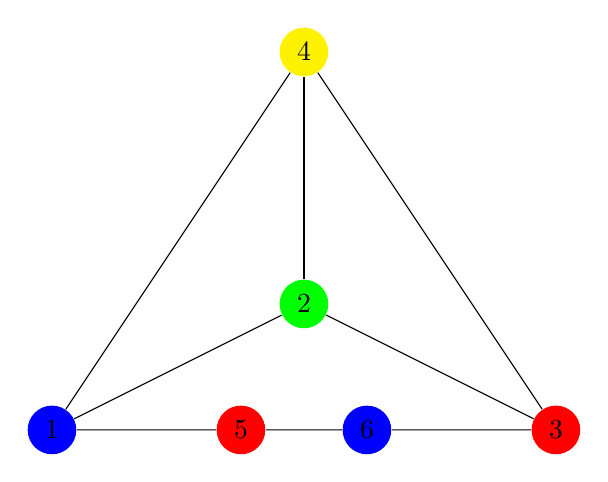
\begin{tikzpicture}
  [scale=.8,auto=left,every node/.style={circle}]
  \node (n1)[fill=blue] at (-1,7) {1};
  \node (n2)[fill=green] at (3,9)  {2};
  \node (n3)[fill=red] at (7,7)  {3};
  \node (n4)[fill=yellow] at (3,13)  {4};
  \node (n5)[fill=red] at (2,7) {5};
  \node (n6)[fill=blue] at (4,7) {6};
 \foreach \from/\to in {n1/n2,n2/n3,n2/n4,n1/n4,n3/n4,n1/n5,n5/n6,n6/n3}
    \draw (\from) -- (\to);
\end{tikzpicture}
\caption{ Proper Coloring the vertices of a graph with 4 colors}\label{10g1}
\end{center}
\end{figure}

\begin{figure}[h]
\begin{center}
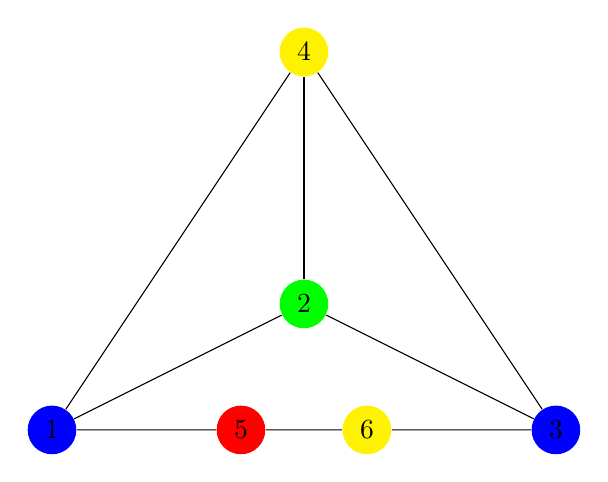
\begin{tikzpicture}
  [scale=.8,auto=left,every node/.style={circle}]
  \node (n1)[fill=blue] at (-1,7) {1};
  \node (n2)[fill=green] at (3,9)  {2};
  \node (n3)[fill=blue] at (7,7)  {3};
  \node (n4)[fill=yellow] at (3,13)  {4};
  \node (n5)[fill=red] at (2,7) {5};
  \node (n6)[fill=yellow] at (4,7) {6};
 \foreach \from/\to in {n1/n2,n2/n3,n2/n4,n1/n4,n3/n4,n1/n5,n5/n6,n6/n3}
    \draw (\from) -- (\to);
\end{tikzpicture}
\caption{ Proper Coloring the vertices of a graph with 3 colors colors}\label{10g2}
\end{center}
\end{figure}

Ajur further stated that 3 colors are needed a vertices 1, 2 and 4 are mutually adjacent and those vertices need 3 different colors. 
Rishnak asked Ajur to properly color the graph $K_{3,3}$, a complete bipartite graph. Ajur jumped at the opportunity and showed a 2 coloring of this graph \ref{10g3}
\begin{figure}
\begin{center}
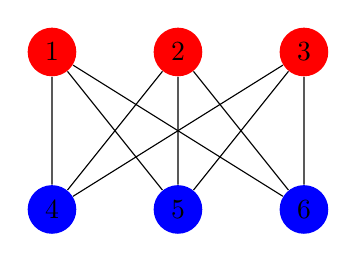
\begin{tikzpicture}
  [scale=.4,auto=left,every node/.style={circle}]
  \node (n1)[fill=red] at (1,7) {1};
  \node (n2)[fill=red] at (5,7)  {2};
  \node (n3)[fill=red] at (9,7) {3};
  \node (n4) [fill=blue] at (1,2)  {4};
  \node (n5) [fill=blue] at (5,2) {5};
  \node (n6)[fill=blue] at (9,2)  {6};
 
  
   \foreach \from/\to in {n1/n6,n1/n4,n1/n5,n2/n6,n2/n4,n2/n5,n3/n4,n3/n5,n3/n6}
    \draw (\from) -- (\to);
    \end{tikzpicture}
\caption{ Two coloring of a Bipartite Graph with 6 vertices and 9 edges, denoted by $K_{3,3}$}\label{10g3}
\end{center}
\end{figure}

Ajur further said that any bipartite graph Vertices are partitioned into two sets $A$ and $B$ and the edges always go from one set, $A$, to the other set, $B$. Ajur further stated that all the vertices in $A$ can be colored with one color, say, red and all the vertices in $B$ can be colored with another color, say blue. Since all tress are also bipartite graphs (contains cycles of even length (=0)), trees can be colored with just two colors. He showed an example \ref{10g4}. Coloring of trees reminded Ajur of the beautiful fall colors one sees in the trees!
\begin{figure}
\begin{center}

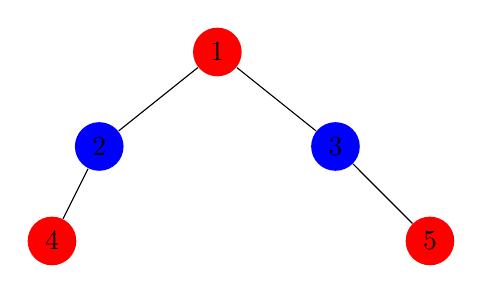
\begin{tikzpicture}
  [scale=.6,auto=left,every node/.style={circle}]
  \node (n1)[fill=red] at (5.5,7) {1};
  \node (n2)[fill=blue] at (3,5)  {2};
  \node (n3)[fill=blue] at (8,5)  {3};
  \node (n4)[fill=red] at (2,3) {4};
  \node (n5)[fill=red] at (10,3)  {5};


  \foreach \from/\to in {n1/n2,n1/n3,n2/n4,n3/n5}
    \draw (\from) -- (\to);

\end{tikzpicture}

\caption{Two coloring of a tree }\label{10g4}
\end{center}
\end{figure}

Ajur was getting curious - He asked Rishnak, "Can one color edges too? How are adjacent edges defined". Rishnak was happy that Ajur was asking the right questions. Rishnak thought to himself that asking the right questions is as important as getting the solutions to those questions. Rishnak answered Ajur that two edges are adjacent if tere are incident on the same vertex. For example consider the graph shown in Figure \ref{10g5},
edge $e1$ is adjacent to $e2$ (both are incident at vertex 1) and to $e3$, $e4$ and $e5$ as all these edges are incident at vertex 2. Four edge coloring of this graph is shown in Figure \ref{10g5}. 

\begin{figure}
\begin{center}

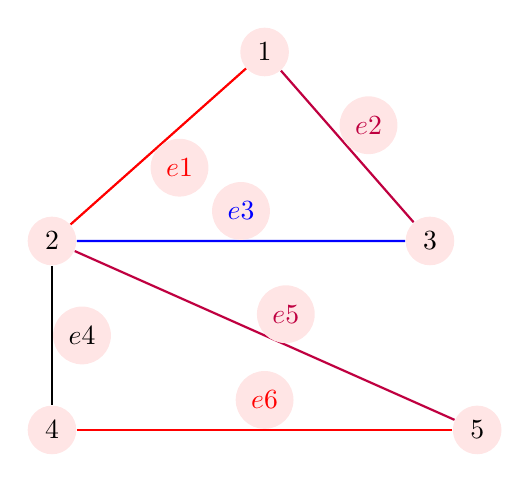
\begin{tikzpicture}
  [scale=.6,auto=left,every node/.style={circle,fill=red!10}]
  \node (n1) at (5.5,9) {1};
  \node (n2) at (1,5)  {2};
  \node (n3) at (9,5)  {3};
  \node (n4) at (1,1) {4};
  \node (n5) at (10,1)  {5};

\path[-,draw,thick]
    (n1) edge [color=red] node {$e1$} (n2)
    (n1) edge [color=purple] node {$e2$} (n3)
    (n2) edge [color=blue] node {$e3$} (n3)
    (n2) edge [color=black] node {$e4$} (n4)
    (n2) edge [color=purple] node {$e5$}  (n5)
    (n4) edge [color=red]node {$e6$}  (n5)
    ;

\end{tikzpicture}

\caption{Four Edge Coloring of a Graph, edge $e1$ is adjacent to $e2$, $e3$,
$e4$ and $e5$}\label{10g5}
\end{center}
\end{figure}

Ajur exclaimed that the maximum degree in this graph is 4 and that is why it needs 4 colors and 4 colors seem to be sufficient. Rishnak smiled said that your observation relating to maximum degree of a graph is good. But it is not really true. Rishnak showed a cycle of length 5, maximum degree is 2, but it needs 3 colors to color its edges.

\begin{figure}
\begin{center}

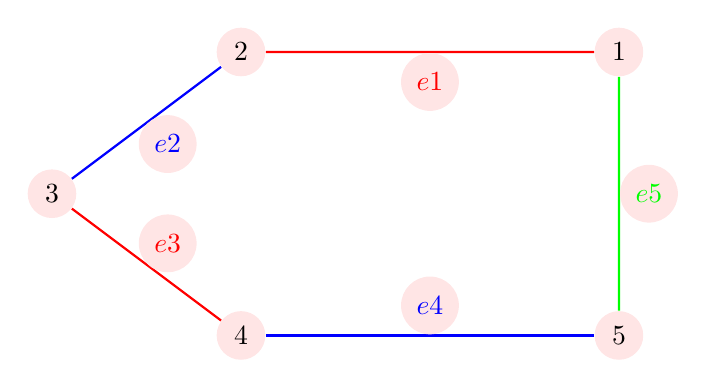
\begin{tikzpicture}
  [scale=.6,auto=left,every node/.style={circle, fill=red!10}]
  \node (n1) at (10,9) {1};
  \node (n2) at (2,9)  {2};
  \node (n3) at (-2,6)  {3};
  \node (n4) at (2,3) {4};
  \node (n5) at (10,3)  {5};

\path[-,draw,thick]
    (n1) edge [color=red] node {$e1$} (n2)
    (n2) edge [color=blue] node {$e2$} (n3)
    (n3) edge [color=red] node {$e3$} (n4)
    (n4) edge [color=blue] node {$e4$} (n5)
    (n1) edge [color=green] node {$e5$}  (n5)
;
\end{tikzpicture}

\caption{Three edge coloring of a cycle of length 5 }\label{10g6}
\end{center}
\end{figure}

Rishnak told Ajur that a graph with maximum degree $\Delta$ can be edge colored with either $\Delta$ or $\Delta+1$ colors. The graphs with regular
graph of degree 3 which needs 4 edge colors are known as Snarks. Ajur exclaimed I have heard of Snarks from a poem by my dad's favorite author Lewis Carroll
\textbf{The Hunting of the Snarks}. Rishnak smiled and said that Graph Theorists have a whimsical sense of humor and since these 4 edge colorable graphs are elusive, they named these classes of graohs as Snarks.
Ajur became curious to find one himself. Ajur asked about Petersen Graph which you asked me to find a Hamiltonian cycle. Rishnak was surprised that Ajur remembered about Petersen Graph. But Rishnak replied to Ajur that Petersen Graph, a regular graph of degree 3, indeed needs 4 colors to color the edges of that graph, see Figure \ref{10g7}
\begin{figure}
\begin{center}
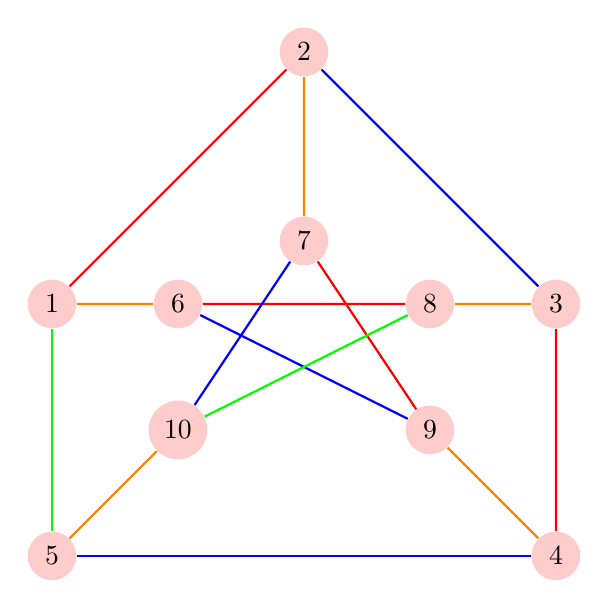
\begin{tikzpicture}
  [scale=.8,auto=left,every node/.style={circle,fill=red!20}]
  \node (n1) at (1,7) {1};
  \node (n2) at (5,11)  {2};
  \node (n3) at (9,7)  {3};
  \node (n4) at (9,3) {4};
  \node (n5) at (1,3) {5};
  \node (n6) at (3,7)  {6};
  \node (n7) at (5,8) {7};
  \node (n8)  at (7,7) {8};
  \node (n9) at (7,5) {9};
  \node (n10) at  (3,5) {10};
 \path[-,draw,thick]
    (n1) edge [color=red]  (n2)
    (n2) edge [color=blue]   (n3)
    (n3) edge [color=red]  (n4)
    (n4) edge [color=blue]  (n5)
    (n1) edge [color=green]  (n5)
    (n7) edge [color=red]   (n9)
    (n9) edge [color=blue]   (n6)
    (n6) edge [color=red]  (n8)
    (n8) edge [color=green]   (n10)
    (n10) edge [color=blue]  (n7)
    (n1) edge [color=orange] (n6)
    (n2) edge [color=orange] (n7)
    (n3) edge [color=orange] (n8)
    (n4) edge [color=orange] (n9)
    (n5) edge [color=orange] (n10)
    
    ;

\end{tikzpicture}
\caption{ 4 edge coloring of Petersen Graph,a regular graph of degree 3  }\label{10g7}
\end{center}
\end{figure}

Map Coloring problem is to color the regions or faces of a planar graph (maps are usually drawn on a plane) so that no two adjacent faces or regions are colored the same.




